% Results narrative. Every number is a macro from generated/numbers.tex (paper/make_assets.py).
% Each paragraph names its source in results/raw/. Negative and null results are reported in place.

\subsection{E1: the sleeper collapse reproduces without the oracle}
On the oracle-free environment, legacy Beta trust detects always-on collusion (median F1 \EoneCraFive{} at
honest fault rate 0.05) but never flags a sleeper within the 300-step attack window (median F1 \EoneTdpFive{};
\EoneTdpTwo{} and \EoneTdpTen{} at fault rates 0.02 and 0.10; Table~\ref{tab:e1}, Fig.~\ref{fig:e1}). Sleepers
accumulate so much positive evidence before switching that the attack window is shorter than the time needed to
pull their trust below 0.5. The collapse is more severe than the 0.11--0.16 reported
in~\cite{padia2025adaptive}; we do not compare magnitudes because that simulator leaked ground truth (E0).
\begin{table}[t]
\centering\scriptsize
\caption{E1: legacy Beta trust on the oracle-free environment. Node-detection F1 over the attack window and at the final step, median [95\% CI] over 30 seeds.}\label{tab:e1}
\resizebox{\columnwidth}{!}{%
\begin{tabular}{llllll}
\toprule
honest fault & F1 CRA (always on) & F1 TDP (sleeper) & final F1 CRA & final F1 TDP & TDP censored sleepers \\
\midrule
0.020000 & 1.000 [1.000, 1.000] & 0.000 [0.000, 0.000] & 1.000 [1.000, 1.000] & 0.000 [0.000, 0.000] & 150/150 \\
0.050000 & 1.000 [1.000, 1.000] & 0.000 [0.000, 0.000] & 1.000 [1.000, 1.000] & 0.000 [0.000, 0.000] & 150/150 \\
0.100000 & 1.000 [1.000, 1.000] & 0.000 [0.000, 0.000] & 1.000 [1.000, 1.000] & 0.000 [0.000, 0.000] & 129/150 \\
\bottomrule
\end{tabular}
}
\end{table}

\begin{figure}[t]\centering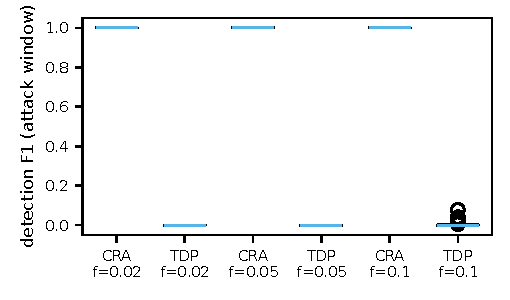
\includegraphics[width=\columnwidth]{e1_collapse.pdf}
\caption{E1: legacy Beta trust, node-detection F1 over the attack window (30 seeds).}\label{fig:e1}\end{figure}

\subsection{E2: SleeperGuard against sleepers}
SleeperGuard is better than legacy Beta in detection F1 in \EtwoSigBetter{} of \EtwoCells{} grid cells
(coalition $\times$ switch time $\times$ intensity; Holm-corrected paired Wilcoxon), worse in \EtwoSigWorse{}.
Median detection delay is \EtwoSgDelayMed{} steps versus \EtwoLgDelayMed{} for legacy Beta. The gain is
not uniform: against a \emph{stealthy} sleeper that inverts only 25\% of its votes, median F1 is about one half
(lowest cell median \EtwoSgFOneMin{}; Table~\ref{tab:e2}, Fig.~\ref{fig:e2}), because a node that lies rarely keeps
its Beta trust above 0.5 and is flagged only while quarantined. Invalid commits stayed rare for both
(max per-run rate \EtwoSgInvalid{} vs.\ \EtwoLgInvalid{}): with $\theta=0.667$ and at most 6 of 16 adversaries, the
main damage of this attack is to liveness (valid transactions rejected), which SleeperGuard reduces.
\begin{table}[t]
\centering\scriptsize
\caption{E2: legacy Beta vs SleeperGuard under the sleeper attack (t\_switch=300, honest fault 0.05), median [95\% CI] over 30 seeds. All grid cells and paired tests: results/raw/stats/e2\_sleeperguard.csv.}\label{tab:e2}
\resizebox{\columnwidth}{!}{%
\begin{tabular}{lllllll}
\toprule
coalition & intensity & F1 legacy & F1 SleeperGuard & delay SG (steps) & valid-reject legacy & valid-reject SG \\
\midrule
0.125 & 0.250000 & 0.000 [0.000, 0.000] & 0.484 [0.447, 0.527] & 5.000 [3.750, 6.000] & 0.001 [0.001, 0.001] & 0.001 [0.001, 0.001] \\
0.125 & 1.000000 & 0.000 [0.000, 0.000] & 0.975 [0.973, 0.985] & 0.000 [0.000, 0.750] & 0.004 [0.004, 0.005] & 0.000 [0.000, 0.001] \\
0.188 & 0.250000 & 0.000 [0.000, 0.000] & 0.492 [0.455, 0.517] & 7.000 [5.000, 9.500] & 0.006 [0.005, 0.007] & 0.003 [0.002, 0.003] \\
0.188 & 1.000000 & 0.000 [0.000, 0.000] & 0.989 [0.983, 0.991] & 0.000 [0.000, 1.000] & 0.017 [0.016, 0.018] & 0.001 [0.000, 0.001] \\
0.25 & 0.250000 & 0.000 [0.000, 0.000] & 0.467 [0.453, 0.500] & 6.500 [5.500, 8.500] & 0.030 [0.029, 0.031] & 0.008 [0.007, 0.009] \\
0.25 & 1.000000 & 0.000 [0.000, 0.000] & 0.992 [0.986, 0.994] & 0.000 [0.000, 1.000] & 0.064 [0.061, 0.065] & 0.003 [0.002, 0.003] \\
0.312 & 0.250000 & 0.000 [0.000, 0.000] & 0.477 [0.453, 0.501] & 7.000 [3.500, 8.000] & 0.108 [0.106, 0.110] & 0.023 [0.021, 0.028] \\
0.312 & 1.000000 & 0.000 [0.000, 0.000] & 0.993 [0.990, 0.994] & 0.000 [0.000, 1.000] & 0.215 [0.208, 0.217] & 0.003 [0.003, 0.004] \\
0.375 & 0.250000 & 0.000 [0.000, 0.000] & 0.484 [0.476, 0.515] & 5.750 [5.000, 8.000] & 0.250 [0.245, 0.253] & 0.055 [0.052, 0.061] \\
0.375 & 1.000000 & 0.000 [0.000, 0.000] & 0.994 [0.991, 0.995] & 0.000 [0.000, 1.000] & 0.536 [0.527, 0.542] & 0.006 [0.005, 0.007] \\
\bottomrule
\end{tabular}
}
\end{table}

\begin{figure}[t]\centering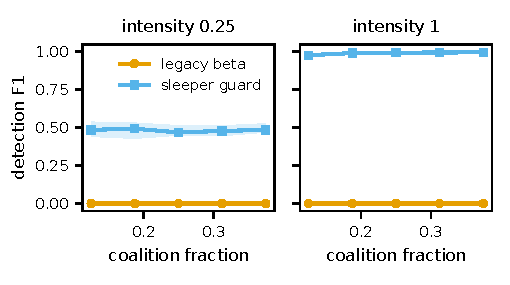
\includegraphics[width=\columnwidth]{e2_sleeperguard.pdf}
\caption{E2: detection F1 vs.\ coalition fraction (median, IQR band), middle switch time.}\label{fig:e2}\end{figure}

\subsection{E3: which component matters}
Against the stealthy sleeper, removing CUSUM drops median F1 from \EthreeFullFOne{} to \EthreeNoCusumFOne{} and raises
mean delay from \EthreeFullDelay{} to \EthreeNoCusumDelay{} steps; removing the two-timescale memory (\EthreeNoTwoFOne{})
or the share cap (\EthreeNoCapFOne{}) changes detection little; removing all three gives \EthreeNoneFOne{}
(Table~\ref{tab:e3}). CUSUM is the active ingredient; the cap matters for the safety bound, not for detection.
The adaptive attacker that replaces the earlier on-off attacker is evaluated in E11.
\begin{table}[t]
\centering\scriptsize
\caption{E3: SleeperGuard ablation, median [95\% CI] over 30 seeds. FQ = honest false quarantines per 1000 node-steps. Paired tests vs full: results/raw/stats/e3\_ablation.csv.}\label{tab:e3}
\resizebox{\columnwidth}{!}{%
\begin{tabular}{lllllll}
\toprule
attack & variant & F1 & delay & honest FQ/1000 & valid-reject & invalid-commit \\
\midrule
CRA (1) & full & 0.995 [0.995, 0.997] & 0.000 [0.000, 0.000] & 0.303 [0.152, 0.303] & 0.001 [0.001, 0.002] & 0.000 [0.000, 0.000] \\
CRA (1) & no-cusum & 1.000 [1.000, 1.000] & 0.000 [0.000, 0.000] & 0.000 [0.000, 0.000] & 0.002 [0.001, 0.002] & 0.000 [0.000, 0.000] \\
CRA (1) & no-two-timescale & 0.995 [0.995, 0.997] & 0.000 [0.000, 0.000] & 0.303 [0.152, 0.303] & 0.001 [0.001, 0.002] & 0.000 [0.000, 0.000] \\
CRA (1) & no-cap & 0.995 [0.995, 0.997] & 0.000 [0.000, 0.000] & 0.303 [0.152, 0.303] & 0.001 [0.001, 0.002] & 0.000 [0.000, 0.000] \\
CRA (1) & none & 1.000 [1.000, 1.000] & 0.000 [0.000, 0.000] & 0.000 [0.000, 0.000] & 0.002 [0.001, 0.002] & 0.000 [0.000, 0.000] \\
TDP (0.25) & full & 0.477 [0.453, 0.501] & 6.300 [4.300, 8.200] & 0.303 [0.227, 0.455] & 0.023 [0.021, 0.028] & 0.000 [0.000, 0.000] \\
TDP (0.25) & no-cusum & 0.047 [0.033, 0.061] & 66.700 [54.800, 90.100] & 0.000 [0.000, 0.000] & 0.058 [0.055, 0.063] & 0.000 [0.000, 0.000] \\
TDP (0.25) & no-two-timescale & 0.472 [0.448, 0.492] & 6.300 [4.300, 8.200] & 0.303 [0.227, 0.455] & 0.020 [0.018, 0.021] & 0.000 [0.000, 0.000] \\
TDP (0.25) & no-cap & 0.477 [0.453, 0.501] & 6.300 [4.300, 8.200] & 0.303 [0.227, 0.455] & 0.023 [0.021, 0.028] & 0.000 [0.000, 0.000] \\
TDP (0.25) & none & 0.000 [0.000, 0.000] & 300.000 [300.000, 300.000] & 0.000 [0.000, 0.000] & 0.056 [0.053, 0.060] & 0.000 [0.000, 0.000] \\
TDP (1) & full & 0.993 [0.990, 0.994] & 0.000 [0.000, 0.800] & 0.303 [0.227, 0.455] & 0.003 [0.003, 0.004] & 0.000 [0.000, 0.000] \\
TDP (1) & no-cusum & 0.998 [0.998, 0.998] & 1.000 [1.000, 1.400] & 0.000 [0.000, 0.000] & 0.004 [0.003, 0.004] & 0.000 [0.000, 0.000] \\
TDP (1) & no-two-timescale & 0.986 [0.983, 0.987] & 0.000 [0.000, 0.800] & 0.303 [0.227, 0.455] & 0.003 [0.003, 0.004] & 0.000 [0.000, 0.000] \\
TDP (1) & no-cap & 0.993 [0.990, 0.994] & 0.000 [0.000, 0.800] & 0.303 [0.227, 0.455] & 0.003 [0.003, 0.004] & 0.000 [0.000, 0.000] \\
TDP (1) & none & 0.930 [0.927, 0.934] & 39.400 [37.400, 41.000] & 0.000 [0.000, 0.000] & 0.034 [0.032, 0.036] & 0.000 [0.000, 0.000] \\
\bottomrule
\end{tabular}
}
\end{table}


\subsection{E4: cost and accuracy of the homomorphic tally}
Over \EfourDecisionsTotal{} random-instance decisions HETally disagreed with the plaintext rule \EfourFlipsTotal{}
times. In the guard-band stress test, decisions agreed for all $|m|\ge$\,\EfourBandMinSafe{} and flips occurred only at
$|m|\le$\,\EfourBandMaxFlip{} (including exact ties). A tally of $k=16$, $T=32$ takes a median \EfourMsZero{}~ms with raw
margins and \EfourMsThree{}~ms with three sign iterations (Table~\ref{tab:e4}, Fig.~\ref{fig:e4}); end-to-end, a step
costs \EfourConsWallZero{}~ms with HE ($s=0$) versus \EfourConsWallPlain{}~ms in plaintext, with
\EfourConsFlipsZero{} decision flips. \textbf{Negative result:} the sign iterations do not hide the margins.
Inverting $p^{(s)}$ recovers every margin to within \EfourLeakErrMax{}, and at most \EfourSatMaxPct{}\% of outputs are
saturated, so the decryptor learns margins in every configuration. The extra iterations add cost without a
measurable privacy gain at these margin magnitudes.
\begin{table}[t]
\centering\scriptsize
\caption{E4: HETally accuracy and cost (CKKS, TenSEAL). Flips = decisions differing from the plaintext rule; m = normalised margin. Latency: median [95\% CI] per tally on the machine in meta.json.}\label{tab:e4}
\resizebox{\columnwidth}{!}{%
\begin{tabular}{lllllllll}
\toprule
sign iters & N & modulus bits (max) & decisions & flips |m|>1e-3 & flips |m|<=1e-3 & max |m| of a flip & ms/tally k=16,T=32 & ct KB \\
\midrule
0 & 8192 & 160 (218) & 3360 & 0 & 0 & 0.00e+00 & 37.554 [35.881, 39.122] & 128 \\
1 & 16384 & 240 (438) & 3360 & 0 & 0 & 0.00e+00 & 221.039 [155.983, 241.716] & 256 \\
2 & 16384 & 320 (438) & 3360 & 0 & 0 & 0.00e+00 & 304.000 [276.540, 433.832] & 256 \\
3 & 16384 & 400 (438) & 3360 & 0 & 0 & 0.00e+00 & 451.207 [415.353, 503.456] & 256 \\
\bottomrule
\end{tabular}
}
\end{table}

\begin{table}[t]
\centering\scriptsize
\caption{E4b: end-to-end runs (TDP, SleeperGuard, 200 steps) with the plaintext vs HE tally on identical seeds.}\label{tab:e4b}
\resizebox{\columnwidth}{!}{%
\begin{tabular}{llllllll}
\toprule
sign iters & backend & seeds & F1 & invalid-commit & valid-reject & HE flips & wall ms/step \\
\midrule
0 & he & 5 & 0.588 [0.538, 0.603] & 0.000 [0.000, 0.000] & 0.020 [0.016, 0.030] & 0 & 32.172 [31.361, 33.035] \\
0 & plain & 5 & 0.588 [0.538, 0.603] & 0.000 [0.000, 0.000] & 0.020 [0.016, 0.030] & 0 & 0.493 [0.295, 0.604] \\
3 & he & 3 & 0.597 [0.538, 0.603] & 0.000 [0.000, 0.000] & 0.021 [0.016, 0.030] & 0 & 471.287 [465.047, 622.256] \\
3 & plain & 3 & 0.597 [0.538, 0.603] & 0.000 [0.000, 0.000] & 0.021 [0.016, 0.030] & 0 & 0.299 [0.225, 0.328] \\
\bottomrule
\end{tabular}
}
\end{table}

\begin{figure}[t]\centering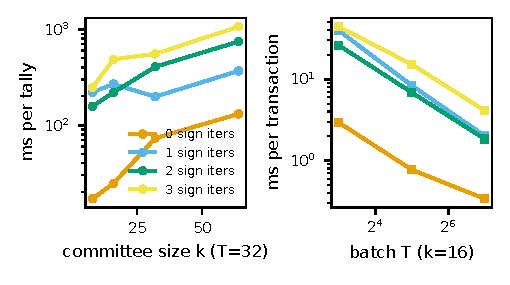
\includegraphics[width=\columnwidth]{e4_he_latency.pdf}
\caption{E4: HETally latency vs.\ committee size and per-transaction cost vs.\ batch size.}\label{fig:e4}\end{figure}

\subsection{E5: scale}
Simulation cost stays small (\EfiveBigWall{}~ms per step and \EfiveBigMem{}~MB peak heap at \EfiveMaxNodes{} nodes, $k=64$),
but \emph{detection does not scale with a fixed committee}: evidence about a node arrives only when it sits on the
committee, so at \EfiveMaxNodes{} nodes \EfiveBigCensoredPct{}\% of sleepers were never flagged within 300 steps (vs.\
\EfiveSmallCensoredPct{}\% at 16 nodes), and the worst cell has median F1 \EfiveMinFOne{} (Table~\ref{tab:e5}).
\begin{table}[t]
\centering\footnotesize\setlength{\tabcolsep}{4pt}
\caption{E5: scale, median over 30 seeds. p95 = simulated step latency (cost model, D7); wall = measured wall-clock per step; heap = peak Python heap of one run. Simulated throughput and p50/p99 latency: results/raw/e5\_scale/runs.csv.}\label{tab:e5}
\begin{tabular}{rrlrrr}
\toprule
$N$ & $k$ & F1 [95\% CI] & p95 ms & wall ms & heap MB \\
\midrule
16 & 8 & 0.83 [0.81, 0.85] & 20.2 & 2.00 & 2 \\
16 & 16 & 0.48 [0.45, 0.50] & 29.8 & 2.49 & 2 \\
64 & 8 & 0.65 [0.60, 0.69] & 20.2 & 2.30 & 3 \\
64 & 16 & 0.82 [0.80, 0.84] & 29.8 & 3.01 & 3 \\
64 & 32 & 0.83 [0.82, 0.85] & 68.2 & 3.47 & 3 \\
64 & 64 & 0.48 [0.47, 0.50] & 221.8 & 5.07 & 4 \\
256 & 8 & 0.24 [0.20, 0.26] & 20.2 & 2.25 & 9 \\
256 & 16 & 0.40 [0.39, 0.43] & 29.8 & 2.53 & 10 \\
256 & 32 & 0.66 [0.65, 0.68] & 68.2 & 3.65 & 10 \\
256 & 64 & 0.81 [0.80, 0.83] & 221.8 & 5.82 & 10 \\
1024 & 8 & 0.06 [0.05, 0.07] & 20.2 & 4.74 & 34 \\
1024 & 16 & 0.12 [0.11, 0.13] & 29.8 & 5.58 & 35 \\
1024 & 32 & 0.22 [0.21, 0.23] & 68.2 & 6.45 & 35 \\
1024 & 64 & 0.42 [0.38, 0.44] & 221.8 & 8.36 & 35 \\
\bottomrule
\end{tabular}
\end{table}


\subsection{E6: audit budget}
Detection degrades gracefully with the audit rate: at audit rate \EsixLowAudit{} SleeperGuard reaches median F1
\EsixSgFOneLowAudit{} against the stealthy sleeper, with mean delay \EsixSgDelayLowAudit{} steps versus \EsixSgDelayFullAudit{}
with every transaction audited (Fig.~\ref{fig:e6}).
\begin{figure}[t]\centering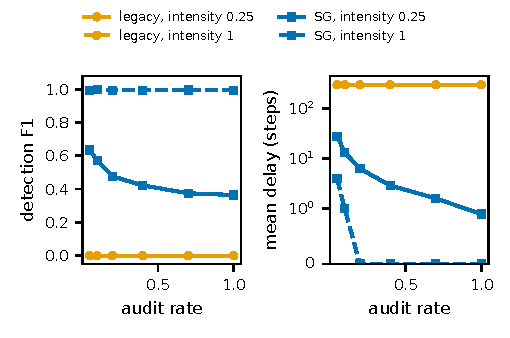
\includegraphics[width=\columnwidth]{e6_audit.pdf}
\caption{E6: detection F1 and delay vs.\ audit rate (median over 30 seeds).}\label{fig:e6}\end{figure}

\subsection{E7: the cost of false quarantines}
With CUSUM calibrated to the true honest fault rate, honest false quarantines per 1000 node-steps are \EsevenFqTwo{},
\EsevenFqFive{}, \EsevenFqTen{} and \EsevenFqTwenty{} at fault rates 0.02, 0.05, 0.10 and 0.20; calibrations for 0.15 and
0.20 lie outside the calibration grid's fault rates and use the nearest (0.10). Misspecified for 0.05 when the true
rate is 0.20, the rate rises to \EsevenFqMisTwenty{} and the valid-reject rate to \EsevenVrMisTwenty{} (Table~\ref{tab:e7}).
Fig.~\ref{fig:e7} shows the delay/false-quarantine trade-off as the alarm threshold varies.
\begin{table}[t]
\centering\scriptsize
\caption{E7: false-positive cost of SleeperGuard vs honest fault rate. 'matched': CUSUM calibrated for the true fault rate; 'fixed\_0.05': calibrated for 0.05 regardless (misspecified). Median [95\% CI], 30 seeds.}\label{tab:e7}
\resizebox{\columnwidth}{!}{%
\begin{tabular}{lllllll}
\toprule
honest fault & calibration & FQ/1000 (no attack) & valid-reject (no attack) & abort rate & F1 (TDP 0.25) & delay (TDP) \\
\midrule
0.000000 & fixed\_0.05 & 0.000 [0.000, 0.000] & 0.000 [0.000, 0.000] & 0.000 [0.000, 0.000] & 0.489 [0.421, 0.509] & 7.000 [4.500, 8.500] \\
0.000000 & matched & 0.000 [0.000, 0.000] & 0.000 [0.000, 0.000] & 0.000 [0.000, 0.000] & 0.678 [0.656, 0.689] & 3.500 [2.000, 4.500] \\
0.020000 & fixed\_0.05 & 0.000 [0.000, 0.000] & 0.000 [0.000, 0.000] & 0.000 [0.000, 0.000] & 0.487 [0.446, 0.512] & 6.400 [4.300, 8.200] \\
0.020000 & matched & 0.365 [0.312, 0.417] & 0.000 [0.000, 0.000] & 0.000 [0.000, 0.000] & 0.673 [0.644, 0.690] & 3.300 [2.000, 5.500] \\
0.050000 & fixed\_0.05 & 0.312 [0.208, 0.312] & 0.000 [0.000, 0.000] & 0.000 [0.000, 0.000] & 0.477 [0.453, 0.501] & 6.300 [4.300, 8.200] \\
0.050000 & matched & 0.312 [0.208, 0.312] & 0.000 [0.000, 0.000] & 0.000 [0.000, 0.000] & 0.477 [0.453, 0.501] & 6.300 [4.300, 8.200] \\
0.100000 & fixed\_0.05 & 2.188 [1.979, 2.448] & 0.006 [0.006, 0.006] & 0.000 [0.000, 0.000] & 0.487 [0.470, 0.503] & 5.900 [3.800, 7.400] \\
0.100000 & matched & 0.625 [0.469, 0.625] & 0.004 [0.004, 0.005] & 0.000 [0.000, 0.000] & 0.386 [0.358, 0.411] & 8.300 [7.000, 13.400] \\
0.150000 & fixed\_0.05 & 5.000 [4.896, 5.104] & 0.040 [0.039, 0.041] & 0.000 [0.000, 0.000] & 0.486 [0.468, 0.496] & 5.300 [3.800, 7.900] \\
0.150000 & matched & 1.927 [1.667, 2.083] & 0.033 [0.032, 0.034] & 0.000 [0.000, 0.000] & 0.414 [0.398, 0.431] & 10.200 [7.300, 14.000] \\
0.200000 & fixed\_0.05 & 8.073 [7.812, 8.385] & 0.122 [0.121, 0.123] & 0.000 [0.000, 0.000] & 0.502 [0.467, 0.520] & 5.900 [4.200, 7.200] \\
0.200000 & matched & 3.594 [3.333, 3.906] & 0.109 [0.108, 0.111] & 0.000 [0.000, 0.000] & 0.461 [0.442, 0.472] & 9.200 [7.000, 12.200] \\
\bottomrule
\end{tabular}
}
\end{table}

\begin{figure}[t]\centering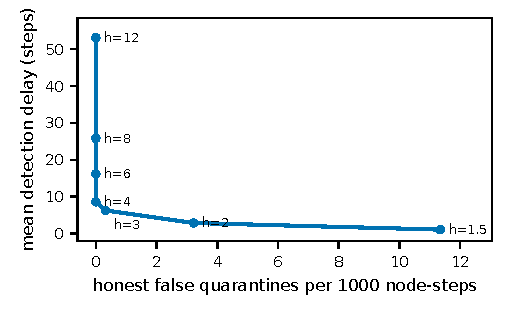
\includegraphics[width=\columnwidth]{e7_tradeoff.pdf}
\caption{E7: detection delay vs.\ honest false quarantines for CUSUM thresholds $h$.}\label{fig:e7}\end{figure}

\subsection{E8 (negative result): hiding the weights does not hinder bribery}
We tested the hypothesis that hiding trust weights hinders an adaptive briber; it is not supported. A briber that sees only the public ledger ranks delegates by how often their votes match
the committed outcome; this reaches a bribed weight share close to that of a briber who sees the weights (largest gap in median share \EeightMaxShareGap{}), and in
\EeightSig{} of \EeightTests{} (backend $\times$ budget) comparisons did the damage (valid-reject rate) differ significantly
after Holm correction. The ledger-based ranking beat random targeting in weight share in \EeightVotesBeatRandom{} of
\EeightVotesRandomTests{} cells (Table~\ref{tab:e8}). Public votes leak influence; encrypting weights alone does not hide it.
\begin{table}[t]
\centering\scriptsize
\caption{E8 (H3): bribery with public weights ('weights') vs hidden weights inferred from the public ledger ('votes') vs random targets. Share = bribed nodes' weight share at bribe time; valid-reject in the 40 steps after bribery. Median [95\% CI], 30 seeds; tests in results/raw/stats/e8\_privacy.csv.}\label{tab:e8}
\resizebox{\columnwidth}{!}{%
\begin{tabular}{llllllll}
\toprule
trust & B & share: weights & share: votes & share: random & valid-reject: weights & valid-reject: votes & valid-reject: random \\
\midrule
legacy beta & 2 & 0.251 [0.251, 0.252] & 0.251 [0.250, 0.251] & 0.125 [0.125, 0.125] & 0.259 [0.249, 0.265] & 0.261 [0.256, 0.268] & 0.047 [0.038, 0.053] \\
legacy beta & 3 & 0.377 [0.376, 0.377] & 0.376 [0.375, 0.376] & 0.250 [0.249, 0.251] & 1.000 [1.000, 1.000] & 1.000 [1.000, 1.000] & 0.260 [0.240, 0.283] \\
legacy beta & 4 & 0.502 [0.502, 0.502] & 0.501 [0.500, 0.501] & 0.374 [0.250, 0.375] & 1.000 [1.000, 1.000] & 1.000 [1.000, 1.000] & 0.939 [0.267, 1.000] \\
sleeper guard & 2 & 0.260 [0.258, 0.263] & 0.250 [0.246, 0.254] & 0.129 [0.122, 0.194] & 0.012 [0.011, 0.015] & 0.013 [0.012, 0.015] & 0.009 [0.006, 0.013] \\
sleeper guard & 3 & 0.390 [0.386, 0.392] & 0.373 [0.321, 0.377] & 0.248 [0.190, 0.292] & 0.035 [0.027, 0.038] & 0.029 [0.026, 0.034] & 0.017 [0.013, 0.028] \\
sleeper guard & 4 & 0.518 [0.513, 0.520] & 0.429 [0.375, 0.502] & 0.371 [0.268, 0.375] & 0.041 [0.036, 0.050] & 0.036 [0.031, 0.043] & 0.034 [0.020, 0.038] \\
\bottomrule
\end{tabular}
}
\end{table}


\subsection{E9: learning vs.\ rules}
All controllers were frozen and evaluated on unseen seeds. The factored independent learners obtained the highest
median reward (\EnineBestLearnerReward{} vs.\ \EnineRuleReward{} for the tuned rule and \EnineFixedReward{} for the fixed
SleeperGuard configuration; Table~\ref{tab:e9}, Fig.~\ref{fig:e9}), and \EnineLearnersBeatRule{} of the three learners beat the rule
significantly. D3P was not significantly better than the rule (reward \EnineDthreeReward{}). \textbf{Caveat:} the reward
(D8) values audited agreement, latency and audit cost, not detection. The best-reward learner shrinks committees and
audits and pays for it with a median detection delay of \EnineBestLearnerDelay{} steps versus \EnineFixedDelay{} for the fixed
configuration, and static DPoS, which detects nothing, scores \EnineDposReward{}. Higher reward here does not mean better
security; a reward that prices detection delay is future work.
\begin{table}[t]
\centering\scriptsize
\caption{E9: frozen controllers on eval seeds 100-129 pooled over six attack settings (180 runs each). Reward is the observable objective (D8); F1 excludes the no-attack setting. Median [95\% CI].}\label{tab:e9}
\resizebox{\columnwidth}{!}{%
\begin{tabular}{llllll}
\toprule
controller & reward & F1 & invalid-commit & valid-reject & throughput (sim.) \\
\midrule
pbft & 0.827 [0.790, 0.857] & 0.000 [0.000, 0.000] & 0.000 [0.000, 0.000] & 0.050 [0.005, 0.108] & 437 \\
static dpos & 0.913 [0.891, 0.922] & 0.000 [0.000, 0.000] & 0.000 [0.000, 0.000] & 0.034 [0.024, 0.068] & 741 \\
majority & 0.859 [0.859, 0.859] & 0.000 [0.000, 0.000] & 0.005 [0.004, 0.005] & 0.000 [0.000, 0.000] & 462 \\
random delegates & 0.864 [0.830, 0.894] & 0.000 [0.000, 0.000] & 0.001 [0.001, 0.002] & 0.099 [0.056, 0.154] & 685 \\
legacy beta & 0.843 [0.823, 0.857] & 0.000 [0.000, 0.000] & 0.000 [0.000, 0.000] & 0.025 [0.005, 0.051] & 450 \\
sleeper guard & 0.857 [0.856, 0.858] & 0.596 [0.548, 0.646] & 0.000 [0.000, 0.000] & 0.005 [0.003, 0.011] & 459 \\
sleeper guard fixed & 0.857 [0.856, 0.858] & 0.596 [0.548, 0.646] & 0.000 [0.000, 0.000] & 0.005 [0.003, 0.011] & 459 \\
rule & 0.856 [0.846, 0.861] & 0.632 [0.559, 0.682] & 0.000 [0.000, 0.000] & 0.015 [0.012, 0.024] & 424 \\
tabular q & 0.904 [0.903, 0.905] & 0.546 [0.422, 0.621] & 0.000 [0.000, 0.000] & 0.016 [0.013, 0.017] & 636 \\
d3p & 0.872 [0.867, 0.876] & 0.656 [0.612, 0.727] & 0.000 [0.000, 0.000] & 0.047 [0.044, 0.049] & 587 \\
marl factored & 0.920 [0.919, 0.922] & 0.693 [0.593, 0.777] & 0.000 [0.000, 0.000] & 0.019 [0.018, 0.021] & 764 \\
\bottomrule
\end{tabular}
}
\end{table}

\begin{figure}[t]\centering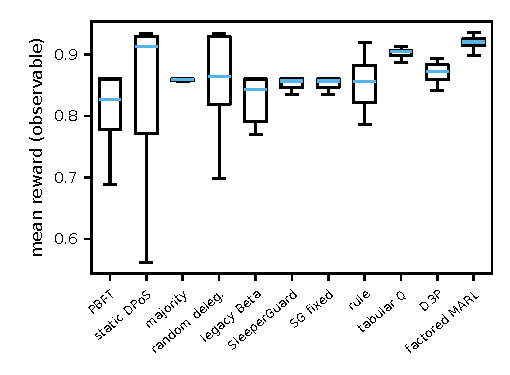
\includegraphics[width=\columnwidth]{e9_controllers.pdf}
\caption{E9: observable reward of frozen controllers on evaluation seeds.}\label{fig:e9}\end{figure}

\subsection{E10: the safety bound under adversarial search}
Across \EtenCells{} (k, c, $\theta$, b) cells the search found \EtenViolations{} violations of
Proposition~\ref{prop:safety} with the exact cap, and every one of the \EtenUnsafeCells{} cells the bound marks unsafe was
broken, so the bound is tight on this grid (Table~\ref{tab:e10}). With the original iterative cap, the tally's cap check
aborted \EtenIterAbortFrac{} of search candidates (exact cap: \EtenExactAbortFrac{}, all from infeasible weight
vectors); safety held only because of the abort.

\textbf{Direct test against the adaptive coalition (E10b).} In the full environment with the exact cap, the
damage-maximising coalition of E11 approved invalid transactions in coordination at lie rates 0.1, 0.3 and 1.0.
For coalitions the bound marks safe ($b\le5$ of 16), no run committed an invalid transaction: \EtenEnvBreachSafeZero{} of
\EtenEnvRunsSafeZero{} runs without honest faults and \EtenEnvBreachSafeFive{} of \EtenEnvRunsSafeFive{} with honest fault
rate 0.05. Above the bound ($b\ge6$), \EtenEnvBreachUnsafe{} of \EtenEnvRunsUnsafe{} runs committed at least one invalid
transaction (max rate \EtenEnvMaxInvalidUnsafe{}), all of them with honest faults present: the faulty honest approvals
are what carry an above-bound coalition over $\theta$, as the faults clause of the proposition predicts. The proposition
therefore needed no change; its honest-fault term is not vacuous (Table~\ref{tab:e10b}).
\begin{table}[t]
\centering\scriptsize
\caption{E10: adversarial search against the capped-influence bound (paper/proof.md). A violation = a commit forced with b below the bound.}\label{tab:e10}
\resizebox{\columnwidth}{!}{%
\begin{tabular}{llllll}
\toprule
k & c & theta & bound: safe for b <= & smallest b that forced a commit & violations \\
\midrule
8 & 1.500000 & 0.500000 & 2 & 3 & 0 \\
8 & 1.500000 & 0.667000 & 3 & 4 & 0 \\
8 & 1.500000 & 0.800000 & 4 & 5 & 0 \\
8 & 2.000000 & 0.500000 & 1 & 2 & 0 \\
8 & 2.000000 & 0.667000 & 2 & 3 & 0 \\
8 & 2.000000 & 0.800000 & 3 & 4 & 0 \\
8 & 3.000000 & 0.500000 & 1 & 2 & 0 \\
8 & 3.000000 & 0.667000 & 1 & 2 & 0 \\
8 & 3.000000 & 0.800000 & 2 & 3 & 0 \\
16 & 1.500000 & 0.500000 & 5 & 6 & 0 \\
16 & 1.500000 & 0.667000 & 7 & 8 & 0 \\
16 & 1.500000 & 0.800000 & 8 & 9 & 0 \\
16 & 2.000000 & 0.500000 & 3 & 4 & 0 \\
16 & 2.000000 & 0.667000 & 5 & 6 & 0 \\
16 & 2.000000 & 0.800000 & 6 & 7 & 0 \\
16 & 3.000000 & 0.500000 & 2 & 3 & 0 \\
16 & 3.000000 & 0.667000 & 3 & 4 & 0 \\
16 & 3.000000 & 0.800000 & 4 & 5 & 0 \\
32 & 1.500000 & 0.500000 & 10 & 11 & 0 \\
32 & 1.500000 & 0.667000 & 14 & 15 & 0 \\
32 & 1.500000 & 0.800000 & 17 & 18 & 0 \\
32 & 2.000000 & 0.500000 & 7 & 8 & 0 \\
32 & 2.000000 & 0.667000 & 10 & 11 & 0 \\
32 & 2.000000 & 0.800000 & 12 & 13 & 0 \\
32 & 3.000000 & 0.500000 & 5 & 6 & 0 \\
32 & 3.000000 & 0.667000 & 7 & 8 & 0 \\
32 & 3.000000 & 0.800000 & 8 & 9 & 0 \\
\bottomrule
\end{tabular}
}
\end{table}

\begin{table}[t]
\centering\scriptsize
\caption{E10b: full environment, exact cap ($k=16$, $c=2$, $	heta=0.667$; bound safe for $b\le5$), damage-maximising coalition approving invalid transactions at lie rates 0.1/0.3/1.0, 30 seeds each.}\label{tab:e10b}
\resizebox{\columnwidth}{!}{%
\begin{tabular}{llllll}
\toprule
b & honest fault & bound says safe & runs with an invalid commit & max invalid-commit rate & median F1 \\
\midrule
1 & 0.000000 & True & 0/9 & 0.0000 & 0.28 \\
1 & 0.050000 & True & 0/9 & 0.0000 & 0.21 \\
2 & 0.000000 & True & 0/9 & 0.0000 & 0.17 \\
2 & 0.050000 & True & 0/9 & 0.0000 & 0.11 \\
3 & 0.000000 & True & 0/9 & 0.0000 & 0.19 \\
3 & 0.050000 & True & 0/9 & 0.0000 & 0.06 \\
4 & 0.000000 & True & 0/9 & 0.0000 & 0.17 \\
4 & 0.050000 & True & 0/9 & 0.0000 & 0.17 \\
5 & 0.000000 & True & 0/9 & 0.0000 & 0.33 \\
5 & 0.050000 & True & 0/9 & 0.0000 & 0.08 \\
6 & 0.000000 & False & 0/9 & 0.0000 & 0.16 \\
6 & 0.050000 & False & 0/9 & 0.0000 & 0.10 \\
7 & 0.000000 & False & 0/9 & 0.0000 & 0.20 \\
7 & 0.050000 & False & 0/9 & 0.0000 & 0.10 \\
8 & 0.000000 & False & 0/9 & 0.0000 & 0.17 \\
8 & 0.050000 & False & 4/9 & 0.0014 & 0.04 \\
\bottomrule
\end{tabular}
}
\end{table}


\subsection{E11: a damage-maximising adaptive coalition}
For each defence we searched lie rate (0.05--1.0), coalition size (2--8 of 16) and target (approve invalid only, or
invert) on seeds 30--39 and kept the configuration with the highest invalid-commit rate. Against every defence the search
chose the largest coalition (\EelevenBSgFull{} of 16, i.e.\ above the bound) approving invalid transactions, at lie rate
\EelevenRateSgFull{} against full SleeperGuard (Table~\ref{tab:e11}). On evaluation seeds the median invalid-commit rate
was \EelevenInvalidSgFull{} with full SleeperGuard versus \EelevenInvalidLegacyBeta{} with legacy Beta and
\EelevenInvalidSgNone{} with all SleeperGuard components removed. \textbf{SleeperGuard does not detect this attacker
well}: median F1 \EelevenFOneSgFull{} (legacy Beta \EelevenFOneLegacyBeta{}; without CUSUM \EelevenFOneSgNoCusum{}). What
limits the damage is coalition size, not detection: for coalitions below the bound, full SleeperGuard had
\EelevenSgBelowBoundBreach{} invalid commits in \EelevenSgBelowBoundRuns{} runs.
\begin{table}[t]
\centering\scriptsize
\caption{E11: each defence against the damage-maximising coalition chosen by search on seeds 30-39 (lie rate, coalition size b of 16, target), evaluated on seeds 100-129. Median [95\% CI].}\label{tab:e11}
\resizebox{\columnwidth}{!}{%
\begin{tabular}{llllllll}
\toprule
defence & attacker lie rate & b & target & invalid-commit & valid-reject & F1 & runs w/ invalid commit \\
\midrule
legacy beta & 0.500000 & 8 & invalid & 0.002 [0.002, 0.003] & 0.000 [0.000, 0.000] & 0.000 [0.000, 0.000] & 30/30 \\
sg full & 0.500000 & 8 & invalid & 0.001 [0.000, 0.001] & 0.001 [0.000, 0.001] & 0.240 [0.224, 0.253] & 26/30 \\
sg no cusum & 0.500000 & 8 & invalid & 0.001 [0.001, 0.001] & 0.000 [0.000, 0.000] & 0.003 [0.002, 0.005] & 30/30 \\
sg no two timescale & 0.300000 & 8 & invalid & 0.001 [0.001, 0.001] & 0.000 [0.000, 0.000] & 0.129 [0.114, 0.142] & 28/30 \\
sg no cap & 0.500000 & 8 & invalid & 0.001 [0.000, 0.001] & 0.000 [0.000, 0.001] & 0.240 [0.224, 0.253] & 26/30 \\
sg none & 0.300000 & 8 & invalid & 0.001 [0.001, 0.002] & 0.000 [0.000, 0.000] & 0.000 [0.000, 0.000] & 29/30 \\
\bottomrule
\end{tabular}
}
\end{table}


\subsection{E12: detection versus lie rate}
With CUSUM calibrated on seeds 20--29 only, SleeperGuard's median F1 rises from \EtwelveFOneLow{} at lie rate
\EtwelveLowRate{} to \EtwelveFOneHigh{} at lie rate 1.0, first reaching 0.5 at lie rate \EtwelveHalfRate{}; legacy Beta
detects nothing below lie rate 0.75. The honest false-quarantine rate on the same runs stays at a median of at most
\EtwelveFqMax{} per 1000 node-steps across all lie rates (Fig.~\ref{fig:e12}). An attacker that lies on fewer than
\EtwelveHalfRate{} of its votes is therefore detected less than half the time.
\begin{figure}[t]\centering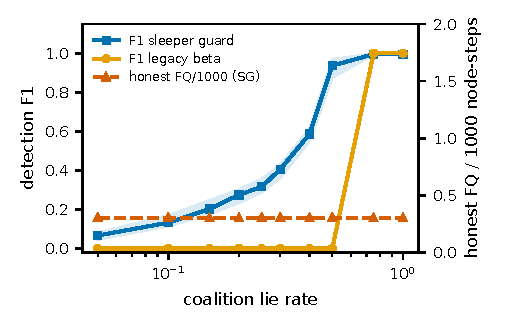
\includegraphics[width=\columnwidth]{e12_lierate.pdf}
\caption{E12: detection F1 (left axis, median and IQR) and honest false quarantines (right axis) vs.\ coalition lie rate.}\label{fig:e12}\end{figure}
